% 
\def\xa{cos(35)}
\def\ya{sin(35)}
\def\xb{cos(135)}
\def\yb{sin(135)}
\def\theta{100}
% 
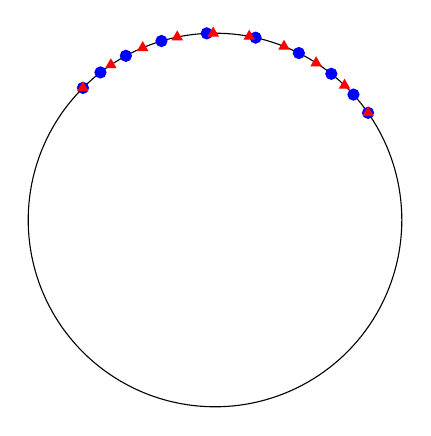
\begin{tikzpicture}
    \begin{axis}[
    hide axis,
    axis equal,
    axis equal image,
    ]
    %\def\PI{3.14159265359}
    \addplot[
        domain=0:360,
        samples=180,
        no marks,
    ]
    ({cos(x)}, {sin(x)});
    % 
    \addplot[
        domain=0:1,
        samples=10,
        only marks,
        mark=*,
        blue,
    ]
    ({((1-x)*\xa + x * \xb) / sqrt(((1-x)*\xa + x * \xb)*((1-x)*\xa + x * \xb) + ((1-x)*\ya + x * \yb)*((1-x)*\ya + x * \yb))}, {((1-x)*\ya + x * \yb) / sqrt(((1-x)*\xa + x * \xb)*((1-x)*\xa + x * \xb) + ((1-x)*\ya + x * \yb)*((1-x)*\ya + x * \yb))});
    % 
    \addplot[
        domain=0:1,
        samples=10,
        only marks,
        mark=triangle*,
        red,
    ]
    ({sin((1-x)*\theta)/sin(\theta)*\xa+sin(x*\theta)/sin(\theta) * \xb},
     {sin((1-x)*\theta)/sin(\theta)*\ya+sin(x*\theta)/sin(\theta) * \yb});
    \end{axis}
\end{tikzpicture}